\begin{adjustwidth*}{}{-2.25in}
\textbf{{\large Exercises}}
\setlength{\columnsep}{25pt}
\begin{multicols*}{2}
\noindent Terms and Concepts \small
\begin{enumerate}[1)]
\item T/F: A solid of revolution is formed by revolving a shape around an axis.
\item T/F: The Shell Method can only be used when the Washer Method fails.
\item T/F: The Shell Method works by integrating cross--sectional areas of a solid.
\item T/F: When finding the volume of a solid of revolution that was revolved around a vertical axis, the Shell Method integrates
with respect to $x$.
\end{enumerate} 

\noindent {\normalsize Problems} \small

\noindent{\bf In Exercises 5--8, a region of the Cartesian plane is shaded. Use the Shell Method to find the volume of the solid of revolution formed by revolving the region about the $y$-axis.}

\begin{enumerate}[1),resume]
\item \begin{minipage}{\linewidth}\centering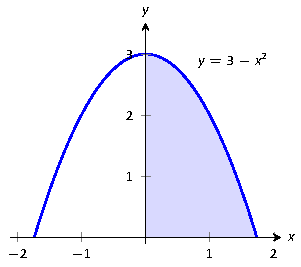
\includegraphics{figures/fig07_02_ex_09}\end{minipage}
\item \begin{minipage}{\linewidth}\centering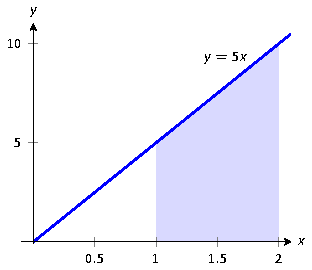
\includegraphics{figures/fig07_02_ex_06}\end{minipage}
\item \begin{minipage}{\linewidth}\centering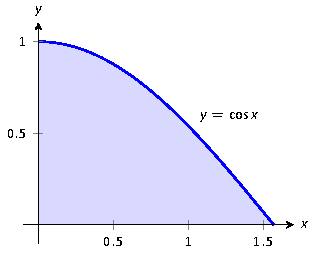
\includegraphics{figures/fig07_02_ex_07}\end{minipage}
\item \begin{minipage}{\linewidth}\centering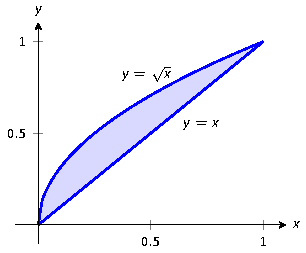
\includegraphics{figures/fig07_02_ex_04}\end{minipage}

%\item \begin{minipage}{\linewidth}\centering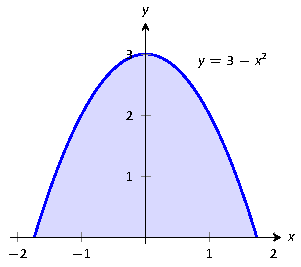
\includegraphics{figures/fig07_02_ex_05}\end{minipage}
\end{enumerate}

\noindent{\bf In Exercises 9--12, a region of the Cartesian plane is shaded. Use the Shell Method to find the volume of the solid of revolution formed by revolving the region about the $x$-axis.}

\begin{enumerate}[1),resume]
\item \begin{minipage}{\linewidth}\centering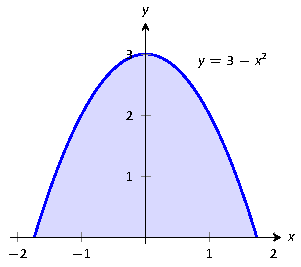
\includegraphics{figures/fig07_02_ex_05}\end{minipage}
\item \begin{minipage}{\linewidth}\centering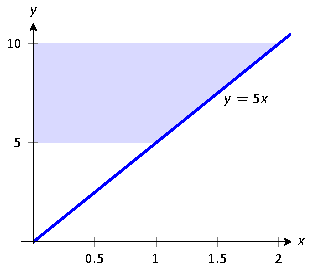
\includegraphics{figures/fig07_02_ex_10}\end{minipage}
\item \begin{minipage}{\linewidth}\centering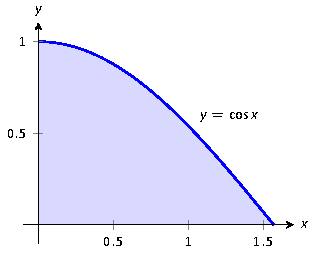
\includegraphics{figures/fig07_02_ex_07}\end{minipage}
\end{enumerate}

%------------------------------------------
% END OF EXERCISES ON FIRST PAGE
%------------------------------------------
\end{multicols*}
\end{adjustwidth*}

\clearpage

\begin{adjustwidth*}{}{-2.25in}
\setlength{\columnsep}{25pt}
\begin{multicols*}{2}\small

\begin{enumerate}[1),start=12]
\item \begin{minipage}{\linewidth}\centering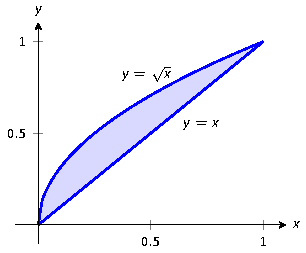
\includegraphics{figures/fig07_02_ex_04}\end{minipage}
\end{enumerate}

\vspace{.25cm}

\noindent{\bf In Exercises 13--18, a region of the Cartesian plane is described. Use the Shell Method to find the volume of the solid of revolution formed by rotating the region about each of the given axes.}

\begin{enumerate}[1),resume]
\item Region bounded by: $y=\sqrt{x}$, $y=0$ and $x=1$.

Rotate about:

\noindent%
\begin{minipage}[t]{.5\linewidth}
\begin{enumerate}
\item		the $y$-axis
\item		$x=1$
\end{enumerate}
\end{minipage}
\begin{minipage}[t]{.5\linewidth}
\begin{enumerate}\addtocounter{enumii}{2}
\item		the $x$-axis
\item		$y=1$
\end{enumerate}
\end{minipage}

\item Region bounded by: $y=4-x^2$ and $y=0$.

Rotate about:

\noindent%
\begin{minipage}[t]{.5\linewidth}
\begin{enumerate}
\item		$x=2$
\item		$x=-2$
\end{enumerate}
\end{minipage}
\begin{minipage}[t]{.5\linewidth}
\begin{enumerate}\addtocounter{enumii}{2}
\item		the $x$-axis
\item		$y=4$
\end{enumerate}
\end{minipage}

\item The triangle with vertices $(1,1)$, $(1,2)$ and $(2,1)$.

Rotate about:

\noindent%
\begin{minipage}[t]{.5\linewidth}
\begin{enumerate}
\item		the $y$-axis
\item		$x=1$
\end{enumerate}
\end{minipage}
\begin{minipage}[t]{.5\linewidth}
\begin{enumerate}\addtocounter{enumii}{2}
\item		the $x$-axis
\item		$y=2$
\end{enumerate}
\end{minipage}

\item Region bounded by $y=x^2-2x+2$ and $y=2x-1$.

Rotate about:

\noindent%
\begin{minipage}[t]{.5\linewidth}
\begin{enumerate}
\item		the $y$-axis
\item		$x=1$
\end{enumerate}
\end{minipage}
\begin{minipage}[t]{.5\linewidth}
\begin{enumerate}\addtocounter{enumii}{2}
%\item		the $y$-axis
\item		$x=-1$
\end{enumerate}
\end{minipage}

\item Region bounded by $y=1/\sqrt{x^2+1}$, $x=-1$, $x=1$ and the $x$-axis.

Rotate about:

\noindent%
\begin{minipage}[t]{.5\linewidth}
\begin{enumerate}
\item		the $y$-axis
\item		$x=1$
\end{enumerate}
\end{minipage}
\begin{minipage}[t]{.5\linewidth}
\begin{enumerate}\addtocounter{enumii}{2}
%\item		the $y$-axis
\item		$y=-1$
\end{enumerate}
\end{minipage}

\item Region bounded by $y=2x$, $y=x$ and $x=2$.

Rotate about:

\noindent%
\begin{minipage}[t]{.5\linewidth}
\begin{enumerate}
\item		the $y$-axis
\item		$x=2$
\end{enumerate}
\end{minipage}
\begin{minipage}[t]{.5\linewidth}
\begin{enumerate}\addtocounter{enumii}{2}
\item		the $x$-axis
\item		$y=4$
\end{enumerate}
\end{minipage}

\end{enumerate}

%---------------------------------------------
% END OF EXERCISES ON SECOND PAGE
%---------------------------------------------
\end{multicols*}
\end{adjustwidth*}

\afterexercises